    En este anexo se describe como se trabaja con el protocolo de comunicación a bajo nivel para codificar el paso de mensajes entre los servos G15 Cube y el microcontrolador. 
    \\
    
    Antes de describir el formato de la información cabe destacar que en todo momento la información enviada irá codificada en formato hexadecimal, para los paquetes enviados como recibidos desde el microcontrolador. Todos los paquetes, tanto los enviados a los servos como la respuesta por parte de los mismos tendrán en común la siguiente información:
    
    \begin{itemize}
    	\item Encabezado: Los primeros dos bytes del mensaje estarán compuestos por encabezado que será el que marque el inicio del mensaje. Estos bytes serán: 0xFF 0xFF
    	\item Un fin de mensaje: El último byte del mensaje estará marcado por un valor llamado \ingles{CheckSum} que será el encargado de verificar que todo el paquete ha llegado correctamente. El \ingles{CheckSum} es el inverso del valor binario de la suma de todos los bytes enviados a excepción del encabezado y el propio \ingles{CheckSum}. En la figura \completar se puede ver un ejemplo de como se calcula dicho valor.
    \end{itemize}
    
    \completarCon{Ejemplo de como se calcula el checksum}
    
    En los paquetes que se envíen a los servos la información se codificará de la siguiente manera concreta:
    
    \begin{itemize}
    	\item Bytes 0 y 1 para el encabezado.
    	\item Byte 2 codifica el ID del servo al que se quiere enviar la acción. De forma general se puede utilizar la dirección 0xFE (en hexadecimal) para enviar el mensaje a todos los servos conectados.
    	\item Byte 2 codifica la longitud del mensaje. Contando a partir del encabezado y el ID (excluyendo ambos) el número de bytes que se envían. De esta forma, al recibirse el paquete se podrá identificar el inicio del mismo, a que servo va dirigido (el resto ignorarán el paquete) y cuantos bytes tendrá que leer el aludido. Por supuesto el último byte de la cadena será el ya mencionado \ingles{CheckSum} cuyo valor tendrá que coincidir con el esperado al analizar la cadena.
    	\item Byte 3 codifica la instrucción que se desea realizar. Sobre la memoria de los servos se podrán hacer operaciones de lectura y escritura de distinta manera. Se pueden ver las diferentes instrucciones posibles en la tabla \ref{tab:g15_instructions}. Serán explicadas posteriormente más en detalle.
    	\item Bytes del 4 al N: Parámetros que se quieran enviar al servo.
    	\item Byte N+1: \ingles{CheckSum}
    \end{itemize}
    
    En la figura \ref{fig:app:registrosg15:comunicacion_mensaje} se puede ver representado, a modo de resumen gráfico, este esquema de información genérico.	
    
    \begin{figure}[H]
    	\centering
    	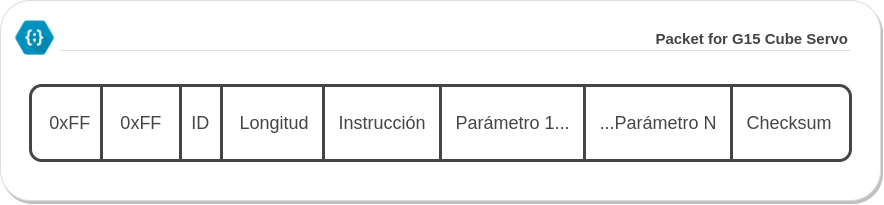
\includegraphics[width=0.9\textwidth]{figuras/Imagenes_SW/Packet_G15.png}   
    	\caption{Paquete de información genérico para comunicar con los Servos G15 Cube}
    	\label{fig:app:registrosg15:comunicacion_mensaje}
    \end{figure}
	

	\begin{table}[htbp]
		\centering
		\caption{Resumen de las instrucciones aceptadas por los Cytron G15 Cube servo}
		\label{tab:g15_instructions}
		\begin{center}
			\begin{tabular}{|c|c|c|}
			\hline
			\textbf{Instrucción} & \textbf{Valor Hex.} & \textbf{Comentarios} \\
			\hline
			iPING & 0x01 & Solicita un paquete con el estado del servo \\
			\hline
			iREAD\_DATA & 0x02 & Lee información de la memoria del servo \\
			\hline
			iWRITE\_DATA & 0x03 & Escribe información en la memoria del servo \\
			\hline
			iREG\_WRITE & 0x04 & Escribe sobre la memoria y hasta que llega la acción \ingles{ACTION} para ejecutar dichos cambios \\
			\hline
			iACTION & 0x05 & Activa la acción codificada con la instrucción \ingles{REG\_WRITE} \\
			\hline
			iRESET & 0x06 & Resetea la memoria a los valores por defecto \\
			\hline
			iSYNC\_WRITE & 0x83 & Para escribir simultáneamente información sobre varios servos \\
			\hline
			\end{tabular}
		\end{center}
	\end{table}	
	
	La respuesta por parte de los servos tiene también una estructura general que se detalla a continuación byte a byte:
	\begin{itemize}
		\item Bytes 0 y 1 de encabezado. Igual que en el caso anterior.
		\item Byte 2 codifica el ID del servo que responde.
		\item Byte 3 codifica la longitud a leer.
		\item Byte 4 sirve para informar de posibles errores en el servo. Cada bit del byte codifica un tipo de error, estando todos a 0 cuando la comunicación y el servo se encuentran buen estado. Estos errores están detallados en la tabla \ref{tab:g15_error}, junto a la máscara en binario que se aplicará a dicho byte para comprobar cada error.
		\item Bytes del 4 al N: Parámetros que envía el servo.
		\item Byte N+1: \ingles{CheckSum}
	\end{itemize}
	
	 En la figura \ref{fig:app:registrosg15:comunicacion_mensaje_from_servo} se puede ver representado, a modo de resumen gráfico, este esquema de información genérico que se ha expuesto previamente.	
	 
	 \begin{figure}[H]
	    	\centering
	    	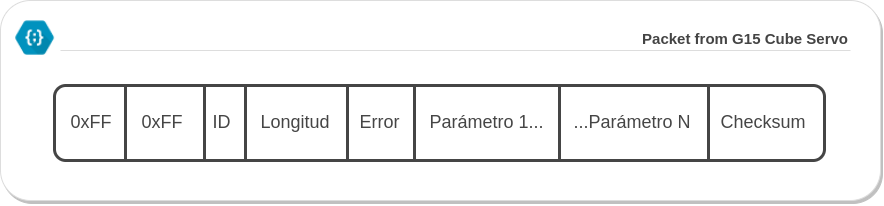
\includegraphics[width=0.9\textwidth]{figuras/Imagenes_SW/Packet_From_G15.png}   
	    	\caption{Paquete de información genérico de retorno de los Servos G15 Cube}
	    	\label{fig:app:registrosg15:comunicacion_mensaje_from_servo}
	 \end{figure}
	
	\begin{table}[htbp]
		\centering
		\caption{Codificación del error de los servos G15 Cube en cada bit del byte de error.}
		\label{tab:g15_error}
		\begin{center}
			\begin{tabular}{|c|c|c|}
				\hline
				\textbf{Bit} & \textbf{Error} & \textbf{Máscara a aplicar} \\
				\hline
				0 & Error en voltaje de entrada & 0X0001 \\
				\hline
				1 & Límite de ángulo & 0X0002 \\
				\hline
				2 & Sobrecalentamiento & 0X0004 \\
				\hline
				3 & Error en el rango pedido & 0X0008 \\
				\hline
				4 & Error en el \ingles{CheckSum} & 0X0010 \\
				\hline
				5 & Sobrecarga & 0X0020 \\
				\hline
				6 & Instrucción incorrecta & 0X0040 \\
				\hline
				7 & - & -  \\
				\hline
			\end{tabular}
		\end{center}
	\end{table}
	
	Aunque como se ha visto anteriormente y se ha detallado en la tabla \ref{tab:g15_error} el servo devuelve un solo byte de error, al leer la información recibida el error, tanto en la librería de Cytron como en la estructura desarrollada para este proyecto este byte se amplia a dos bytes para añadir la posibilidad de nuevos errores en la recepción del paquete de datos. Se pueden ver de forma detallada en la tabla \ref{tab:g15_error_second}, nuevamente junto a la máscara que se aplicará a dicho byte para cada caso. En el byte más bajo queda la información que devuelve el servo y en el más alto la información añadida.
	\\ 
	
	\begin{table}[htbp]
		\centering
		\caption{Codificación del error de comunicación en cada bit del segundo byte de error.}
		\label{tab:g15_error_second}
		\begin{center}
			\begin{tabular}{|c|c|c|}
				\hline
				\textbf{Bit} & \textbf{Error} & \textbf{Máscara a aplicar} \\
				\hline
				8 & Paquete perdido o tiempo de espera superado & 0X0100 \\
				\hline
				9 & Encabezado incorrecto & 0X0200 \\
				\hline
				10 & ID incorrecto & 0X0400 \\
				\hline
				11 & Error en el \ingles{CheckSum} & 0X0800 \\
				\hline
				12 & - & -  \\
				\hline
				13 & - & -  \\
				\hline
				14 & - & -  \\
				\hline
				15 & - & -  \\
				\hline
			\end{tabular}
		\end{center}
	\end{table}
	
	A continuación se detallan las distintas instrucciones que aceptan los Servos, presentadas en la tabla \ref{tab:g15_instructions}.
	\subsection{Petición del estado del servo}
	
	\subsection{Operaciones de lectura}
	
	\subsection{Operaciones de escritura}
	
	\subsection{Operaciones de escritura con activación desacoplada}
	
	\subsection{Operaciones de escritura sobre múltiples servos}


\begin{table}[htbp]
	\caption{Características mas importantes de los Servos G15 de Cytron. Tabla traducida y resumida a los puntos más importantes del Cytron G15 Cube servo User Manual \cite{CytronTechnologies2012} \completarCon{¿esto está bien, hay que poner paginas involucradas?}}
	\label{tab:g15_register}
	\begin{adjustwidth}{-1.9cm}{-1.5cm}
	\begin{tabular}{|c|c|c|c|c|c|c|}
		\hline
		\textbf{Area} & \textbf{\shortstack{Address\\ (Hex)}} & \textbf{Parameter} & \textbf{\shortstack{Read only \\ /Read Write}} & \textbf{\shortstack{Factory\\ default\\ value (Hex)}} & \textbf{\shortstack{Minimum\\ value (Hex)}} & \textbf{\shortstack{Maximum\\ value (Hex)}} \\ \hline
		\multicolumn{ 1}{|c|}{EEPROM} & 0 (0x00) & Model (L) & R & ‘G’ (0x0F) & - & - \\ \cline{ 2- 7}
		\multicolumn{ 1}{|c|}{} & 1 (0x01) & Model(H) & R & 15 (0x47) & - & - \\ \cline{ 2- 7}
		\multicolumn{ 1}{|c|}{} & 2 (0x02) & Firmware Revision & R &  & - & - \\ \cline{ 2- 7}
		\multicolumn{ 1}{|c|}{} & 3 (0x03) & ID & RW & 1 (0x01) & 0 (0x00) & 253 (0xFD) \\ \cline{ 2- 7}
		\multicolumn{ 1}{|c|}{} & 4 (0x04) & Baud Rate & RW & 103 (0x67) & 3 (0x03) & 255 (0xFF) \\ \cline{ 2- 7}
		\multicolumn{ 1}{|c|}{} & 5 (0x05) & Return Delay & RW & 250 (0xFA)  & 1 (0x01)  & 255 (0xFF) \\ \cline{ 2- 7}
		\multicolumn{ 1}{|c|}{} & 6 (0x06) & CW Angle Limit (L) & RW & \multicolumn{ 1}{c|}{ 0 (0x0000) } & \multicolumn{ 1}{c|}{ 0 (0x0000) } & \multicolumn{ 1}{c|}{1087 (0x043F)} \\ \cline{ 2- 4}
		\multicolumn{ 1}{|c|}{} & 7 (0x07) & CW Angle Limit (H) & RW & \multicolumn{ 1}{c|}{} & \multicolumn{ 1}{c|}{} & \multicolumn{ 1}{c|}{} \\ \cline{ 2- 7}
		\multicolumn{ 1}{|c|}{} & 8 (0x08) & CCW Angle Limit (L) & RW & \multicolumn{ 1}{c|}{1087 (0x043F)} & \multicolumn{ 1}{c|}{ 0 (0x0000) } & \multicolumn{ 1}{c|}{1087 (0x043F)} \\ \cline{ 2- 4}
		\multicolumn{ 1}{|c|}{} & 9 (0x09) & CCW Angle Limit (H) & RW & \multicolumn{ 1}{c|}{} & \multicolumn{ 1}{c|}{} & \multicolumn{ 1}{c|}{} \\ \cline{ 2- 7}
		\multicolumn{ 1}{|c|}{} & 10 (0x0A) & Reserved & - & - & - & - \\ \cline{ 2- 7}
		\multicolumn{ 1}{|c|}{} & 11 (0x0B) & Temperature Limit & RW & 70 (0x46) & 0 (0x00) &  \\ \cline{ 2- 7}
		\multicolumn{ 1}{|c|}{} & 12 (0x0C) & Lowest Voltage Limit & RW & 65 (0x41) & 65 (0x41) & 178 (0xB2) \\ \cline{ 2- 7}
		\multicolumn{ 1}{|c|}{} & 13 (0x0D) & Highest Voltage Limit & RW & 150 (0x96)  &  &  \\ \cline{ 2- 7}
		\multicolumn{ 1}{|c|}{} & 14 (0x0E) & Max Torque (L) & RW & \multicolumn{ 1}{c|}{1023 (0x03FF)} & \multicolumn{ 1}{c|}{ 0 (0x0000) } & \multicolumn{ 1}{c|}{1023 (0x03FF)} \\ \cline{ 2- 4}
		\multicolumn{ 1}{|c|}{} & 15 (0x0F) & Max Torque (H) & RW & \multicolumn{ 1}{c|}{} & \multicolumn{ 1}{c|}{} & \multicolumn{ 1}{c|}{} \\ \cline{ 2- 7}
		\multicolumn{ 1}{|c|}{} & 16 (0x10) & Return Packet Enable & RW & 2 (0x02) & 0 (0x00) & 2 (0x02) \\ \cline{ 2- 7}
		\multicolumn{ 1}{|c|}{} & 17 (0x11) & Alarm LED & RW & 36 (0x24) & 0 (0x00) & 127 (0x7F) \\ \cline{ 2- 7}
		\multicolumn{ 1}{|c|}{} & 18 (0x12) & Alarm Shutdown & RW & 36 (0x24) & 0 (0x00) & 127 (0x7F) \\ \cline{ 2- 7}
		\multicolumn{ 1}{|c|}{} & 19 (0x13) & Reserved & - & - & - & - \\ \cline{ 2- 7}
		\multicolumn{ 1}{|c|}{} & 20 (0x14) & Down Calibration (L) & R &  &  &  \\ \cline{ 2- 7}
		\multicolumn{ 1}{|c|}{} & 21 (0x15) & Down Calibration (H) & R &  &  &  \\ \cline{ 2- 7}
		\multicolumn{ 1}{|c|}{} & 22 (0x16) & Up Calibration (L) & R &  &  &  \\ \cline{ 2- 7}
		\multicolumn{ 1}{|c|}{} & 23 (0x17) & Up Calibration (H) & R &  &  &  \\ \hline
		\multicolumn{ 1}{|c|}{RAM} & 24 (0x18) & Torque Enable & RW & 0 (0x00) & 0 (0x00) & 1 (0x01) \\ \cline{ 2- 7}
		\multicolumn{ 1}{|c|}{} & 25 (0x19) & LED & RW & 0 (0x00) & 0 (0x00) & 1 (0x01) \\ \cline{ 2- 7}
		\multicolumn{ 1}{|c|}{} & 26 (0x1A) & CW Compliance Margin & RW & 1 (0x01) & 0 (0x00) & 254(0xFE) \\ \cline{ 2- 7}
		\multicolumn{ 1}{|c|}{} & 27 (0x1B) & CCW Compliance & RW & 1 (0x01) & 0 (0x00) & 254(0xFE) \\ \cline{ 2- 7}
		\multicolumn{ 1}{|c|}{} & 28 (0x1C) & CW Compliance Slope & RW & 32 (0x0020) & 1 (0x01) & 254(0xFE) \\ \cline{ 2- 7}
		\multicolumn{ 1}{|c|}{} & 29 (0x1D) & CCW Compliance Slope & RW & 32 (0x0020) & 1 (0x01) & 254(0xFE) \\ \cline{ 2- 7}
		\multicolumn{ 1}{|c|}{} & 30 (0x1E) & Goal Position (L) & RW & Address 36 & \multicolumn{ 1}{c|}{ 0 (0x0000) } & \multicolumn{ 1}{c|}{1087 (0x043F)} \\ \cline{ 2- 5}
		\multicolumn{ 1}{|c|}{} & 31 (0x1F) & Goal Position (H) & RW & Address 37 & \multicolumn{ 1}{c|}{} & \multicolumn{ 1}{c|}{} \\ \cline{ 2- 7}
		\multicolumn{ 1}{|c|}{} & 32 (0x020) & Moving Speed (L) & RW & \multicolumn{ 1}{c|}{ 0 (0x0000) } & \multicolumn{ 1}{c|}{ 0 (0x0000) } & \multicolumn{ 1}{c|}{1023 (0x03FF)} \\ \cline{ 2- 4}
		\multicolumn{ 1}{|c|}{} & 33 (0x21) & Moving Speed (H) & RW & \multicolumn{ 1}{c|}{} & \multicolumn{ 1}{c|}{} & \multicolumn{ 1}{c|}{} \\ \cline{ 2- 7}
		\multicolumn{ 1}{|c|}{} & 34 (0x22) & Torque Limit (L) & RW & Address 14 & \multicolumn{ 1}{c|}{ 0 (0x0000) } & \multicolumn{ 1}{c|}{1023 (0x03FF)} \\ \cline{ 2- 5}
		\multicolumn{ 1}{|c|}{} & 35 (0x23) & Torque Limit (H) & RW & Address 15 & \multicolumn{ 1}{c|}{} & \multicolumn{ 1}{c|}{} \\ \cline{ 2- 7}
		\multicolumn{ 1}{|c|}{} & 36 (0x24) & Present Position (L) & R & \multicolumn{ 1}{c|}{} & \multicolumn{ 1}{c|}{} & \multicolumn{ 1}{c|}{} \\ \cline{ 2- 4}
		\multicolumn{ 1}{|c|}{} & 37 (0x25) & Present Position (H) & R & \multicolumn{ 1}{c|}{} & \multicolumn{ 1}{c|}{} & \multicolumn{ 1}{c|}{} \\ \cline{ 2- 7}
		\multicolumn{ 1}{|c|}{} & 38 (0x26) & Present Speed (L) & R & \multicolumn{ 1}{c|}{} & \multicolumn{ 1}{c|}{} & \multicolumn{ 1}{c|}{} \\ \cline{ 2- 4}
		\multicolumn{ 1}{|c|}{} & 39 (0x27) & Present Speed (H) & R & \multicolumn{ 1}{c|}{} & \multicolumn{ 1}{c|}{} & \multicolumn{ 1}{c|}{} \\ \cline{ 2- 7}
		\multicolumn{ 1}{|c|}{} & 40 (0x28) & Present Load (L) & R & \multicolumn{ 1}{c|}{} & \multicolumn{ 1}{c|}{} & \multicolumn{ 1}{c|}{} \\ \cline{ 2- 4}
		\multicolumn{ 1}{|c|}{} & 41 (0x29) & Present Load (H) & R & \multicolumn{ 1}{c|}{} & \multicolumn{ 1}{c|}{} & \multicolumn{ 1}{c|}{} \\ \cline{ 2- 7}
		\multicolumn{ 1}{|c|}{} & 42 (0x2A) & Present Voltage & R &  &  &  \\ \cline{ 2- 7}
		\multicolumn{ 1}{|c|}{} & 43 (0x2B) & Present Temperature & R &  &  &  \\ \cline{ 2- 7}
		\multicolumn{ 1}{|c|}{} & 44 (0x2C) & Registered & R & 0 (0x00) & 0 (0x00) & 1 (0x01) \\ \cline{ 2- 7}
		\multicolumn{ 1}{|c|}{} & 45 (0x2D) & Reserved & - & - & - & - \\ \cline{ 2- 7}
		\multicolumn{ 1}{|c|}{} & 46 (0x2E) & Moving & R & 0 (0x00) & 0 (0x00) & 1 (0x01) \\ \cline{ 2- 7}
		\multicolumn{ 1}{|c|}{} & 47 (0x2F) & Lock & RW & 0 (0x00) & 1 (0x01) & 1 (0x01) \\ \cline{ 2- 7}
		\multicolumn{ 1}{|c|}{} & 48 (0x30) & Punch (L) & RW & \multicolumn{ 1}{c|}{32 (0x0020)} & \multicolumn{ 1}{c|}{0 (0x0000)} & \multicolumn{ 1}{c|}{1023 (0x03FF)} \\ \cline{ 2- 4}
		\multicolumn{ 1}{|c|}{} & 49 (0x31) & Punch (H) & RW & \multicolumn{ 1}{c|}{} & \multicolumn{ 1}{c|}{} & \multicolumn{ 1}{c|}{} \\ \hline
	\end{tabular}
\end{adjustwidth}
\end{table}	

